\documentclass{article}

\usepackage{booktabs}
\usepackage{tabularx}
\usepackage{hyperref}
\usepackage{graphicx}
\usepackage{multirow}
\usepackage{pdflscape}
\graphicspath{./diagrams/}

\hypersetup{
    colorlinks=true,       % false: boxed links; true: colored links
    linkcolor=red,          % color of internal links (change box color with linkbordercolor)
    citecolor=green,        % color of links to bibliography
    filecolor=magenta,      % color of file links
    urlcolor=cyan           % color of external links
}

\title{Hazard Analysis\\\progname}

\author{\authname}

\date{}

%% Comments

\usepackage{color}

\newif\ifcomments\commentstrue %displays comments
%\newif\ifcomments\commentsfalse %so that comments do not display

\ifcomments
\newcommand{\authornote}[3]{\textcolor{#1}{[#3 ---#2]}}
\newcommand{\todo}[1]{\textcolor{red}{[TODO: #1]}}
\else
\newcommand{\authornote}[3]{}
\newcommand{\todo}[1]{}
\fi

\newcommand{\wss}[1]{\authornote{blue}{SS}{#1}} 
\newcommand{\plt}[1]{\authornote{magenta}{TPLT}{#1}} %For explanation of the template
\newcommand{\an}[1]{\authornote{cyan}{Author}{#1}}

%% Common Parts

\newcommand{\progname}{Software Engineering} % PUT YOUR PROGRAM NAME HERE
\newcommand{\authname}{Team 8 -- Rhythm Rangers\\
\\ Ansel Chen
\\ Muhammad Jawad
\\ Mohamad-Hassan Bahsoun
\\ Matthew Baleanu
\\ Ahmed Al-Hayali} % AUTHOR NAMES                  

\usepackage{hyperref}
    \hypersetup{colorlinks=true, linkcolor=blue, citecolor=blue, filecolor=blue,
                urlcolor=blue, unicode=false}
    \urlstyle{same}
                                


\begin{document}

\maketitle
\thispagestyle{empty}

~\newpage

\pagenumbering{roman}

\begin{table}[hp]
\caption{Revision History} \label{TblRevisionHistory}
\begin{tabularx}{\textwidth}{llX}
\toprule
\textbf{Date} & \textbf{Developer(s)} & \textbf{Change}\\
\midrule
Date1 & Name(s) & Description of changes\\
Date2 & Name(s) & Description of changes\\
... & ... & ...\\
\bottomrule
\end{tabularx}
\end{table}

~\newpage

\tableofcontents

~\newpage

\pagenumbering{arabic}

\wss{You are free to modify this template.}

\section{Introduction}

\wss{You can include your definition of what a hazard is here.}

\section{Scope and Purpose of Hazard Analysis}

\wss{You should say what \textbf{loss} could be incurred because of the
hazards.}

\section{System Boundaries and Components}
\subsection{Diagrammatic System Characterization}
\begin{center}
    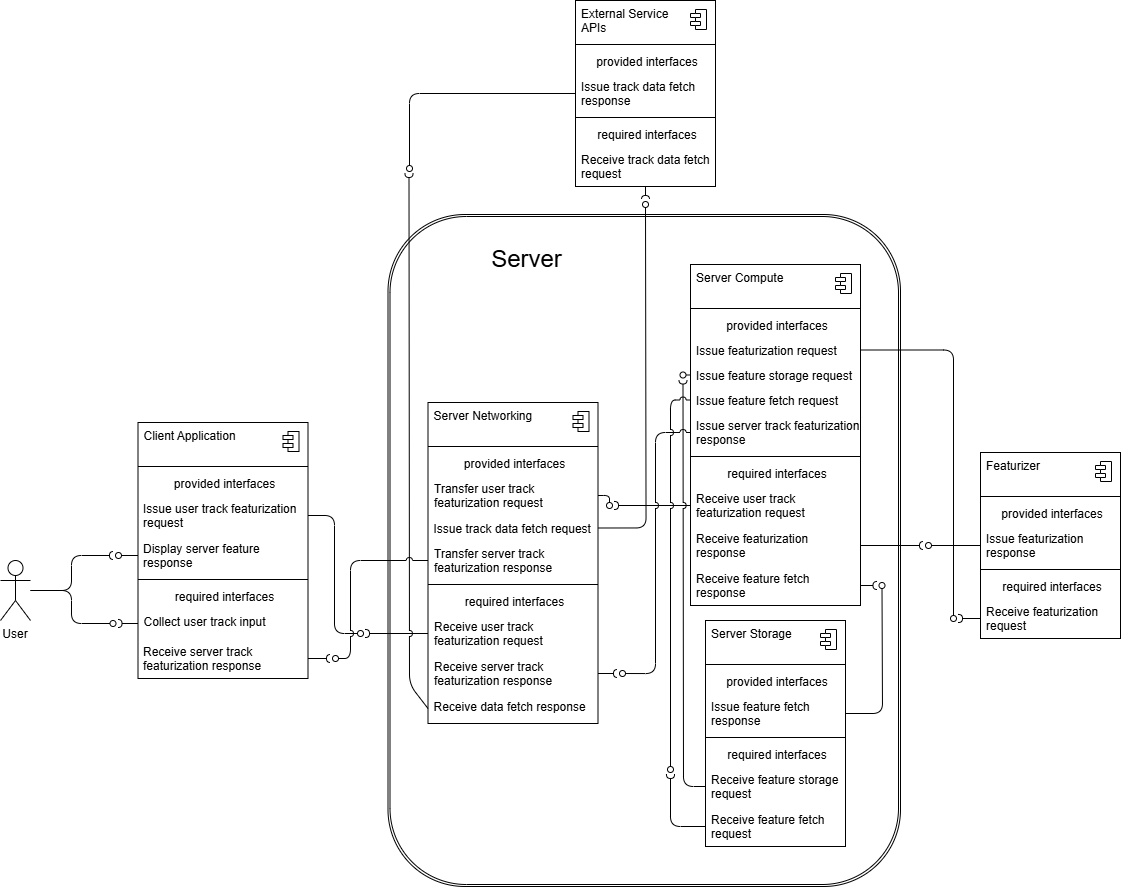
\includegraphics[width=\textwidth]{/diagrams/2_1_system_characterization_diagram.png}
\end{center}
\subsection{System Component Descriptions}
Please refer to table \ref{tbl:sys-cmpnt-desc}.
\begin{table}[h!]
    \centering
    \begin{tabular}{ p{.25\linewidth} || p{.65\linewidth} }
      \textbf{Component Name} & \textbf{Component Description} \\
      \toprule
      \emph{Client Application} & User-facing component through which they can input track information and view track features as system output. \\
      \midrule
      \emph{Server Networking} & Abstract component that represents communication between the server and external components, i.e., the client application and external service APIs. \\
      \midrule
      \emph{Server Compute} & Component that represents the server processing mechanism, i.e., the component that issues the featurization request. \\
      \midrule
      \emph{Server Storage} & Component that represents the server storage, i.e., the database. \\
      \midrule
      \emph{External Service APIs} & Component that represents external service APIs, e.g., the \href{https://developer.spotify.com/}{Spotify API} or \href{https://developers.deezer.com/}{Deezer API}. \\
      \midrule
      \emph{Featurizer} & Component that handles the featurization process.
    \end{tabular}
    \label{tbl:sys-cmpnt-desc}
    \caption{System Component Descriptions}
  \end{table}

\section{Critical Assumptions}

\wss{These assumptions that are made about the software or system.  You should
minimize the number of assumptions that remove potential hazards.  For instance,
you could assume a part will never fail, but it is generally better to include
this potential failure mode.}

\section{Failure Mode and Effect Analysis}

\begin{landscape}
\begin{table}[]
    \scalebox{.45}{
    \begin{tabular}{|l|l|l|l|l|l|}
    \hline
    Component/Design Function & Failure Mode & Effects of Failure & Causes of Failure & Detection & Recommended Action(s) \\ \hline
    \multirow{2}{*}{User Interface App} & Unresponsive UI elements & UI stops responding to user inputs & Poor backend implementation &  & Display a message to the user to refresh the page \\
     &  & User frustration & Poor frontend implementation &  &  \\
    Featurizer & Poor featurization of music & Featurizer returns incorrect or incomplete data to the webapp & Poor implementation of featurizer algorithm &  & Ensure featurizer algorithm is robust and well tested \\
    External Service APIs & API Request Blocked & Service that requires API stops functioning & Hit Music Streaming Provider API rate limit &  & \begin{tabular}[c]{@{}l@{}}- Throttle API requests if there are a large amount of them\\ - minimize the amount of API calls the service makes\\ - fallbacks if API request denied (request post-poned instead of cancelled)\end{tabular} \\
    Version Control System & Merge conflict resolved improperly & Section(s) of documentation are erroneously deleted & Improper merge conflict resolution within github & \begin{tabular}[c]{@{}l@{}}- Regularly Checking Github Repo for integrity\\ - Recompiling the PDF from latex to check for errors before deadlines\\ - Project Supervisor(s) notice during marking\end{tabular} & \begin{tabular}[c]{@{}l@{}}- Use Github Branchrs\\ - Proper Merge Conflict resolution\end{tabular} \\
    \multirow{3}{*}{Server Networking} & Webapp can't connect to server & App gets stuck on current task & Server network module fails &  & Display message to user, attempt to reconnect to the server \\
     &  &  & Server loses power &  & Regularly backup server storage \\
     &  &  & Webapp device network module fails &  &  \\
    \multirow{3}{*}{Server Compute} & Server timeout & No response from the server & Server is overloaded &  & Display message to user to contact system administrator \\
     &  &  & Server power loss &  & Regularly backup server storage \\
     &  &  & Poor computation logic &  & Optimize processing algorithms \\
    \multirow{8}{*}{Server Storage} & Server storage is inaccessible & Server query failure & Storage device failure &  & Display message to user to contact system administrator \\
     &  &  & Server power loss &  & Regularly backup server storage \\
     &  &  &  &  &  \\
     & Duplicate database entries & Compute unit returns incorrect information & Lack of duplicate protection &  & Implement duplicate protection measures \\
     &  &  &  &  & Merge duplicate entries \\
     &  &  &  &  &  \\
     & Data corruption & Compute unit response contains errors or is empty & Server power loss &  & Regularly backup server storage \\
     &  & Data loss & Storage device failure &  &  \\ \hline
    \end{tabular}
    }
\end{table}
\end{landscape}

\wss{The safety requirements in the table do not have to have the prefix SR.
The most important thing is to show traceability to your SRS. You might trace to
requirements you have already written, or you might need to add new
requirements.}
\wss{If no safety requirement can be devised, other mitigation strategies can be
entered in the table, including strategies involving providing additional
documentation, and/or test cases.}

\section{Safety and Security Requirements}

\wss{Newly discovered requirements.  These should also be added to the SRS.  (A
rationale design process how and why to fake it.)}

\section{Roadmap}

\wss{Which safety requirements will be implemented as part of the capstone timeline?
Which requirements will be implemented in the future?}

\newpage{}

\section*{Appendix --- Reflection}

\wss{Not required for CAS 741}

The purpose of reflection questions is to give you a chance to assess your own
learning and that of your group as a whole, and to find ways to improve in the
future. Reflection is an important part of the learning process.  Reflection is
also an essential component of a successful software development process.  

Reflections are most interesting and useful when they're honest, even if the
stories they tell are imperfect. You will be marked based on your depth of
thought and analysis, and not based on the content of the reflections
themselves. Thus, for full marks we encourage you to answer openly and honestly
and to avoid simply writing ``what you think the evaluator wants to hear.''

Please answer the following questions.  Some questions can be answered on the
team level, but where appropriate, each team member should write their own
response:


\begin{enumerate}
    \item What went well while writing this deliverable? 
    \item What pain points did you experience during this deliverable, and how
    did you resolve them?
    \item Which of your listed risks had your team thought of before this
    deliverable, and which did you think of while doing this deliverable? For
    the latter ones (ones you thought of while doing the Hazard Analysis), how
    did they come about?
    \item Other than the risk of physical harm (some projects may not have any
    appreciable risks of this form), list at least 2 other types of risk in
    software products. Why are they important to consider?
\end{enumerate}

\end{document}